\begin{question}[type=exam]{10}
  Consider the production decision of a firm who's production costs are represented by the
  marginal cost $MC$, average variable cost $AVC$, and average total cost $ATC$ curves below.

\begin{itemize}
\item  Suppose that in the \textbf{short-run}, the perfectly competitive market price is at a level represented by the horizontal line labelled $P$.
  Illustrate how much quantity the firm will produce in the short run on the graph.
  \item Now explain what will happen to this market in the \textbf{long-run} if firms are allowed to enter or exit.
  Use the graph to explain your answer.
\end{itemize} 

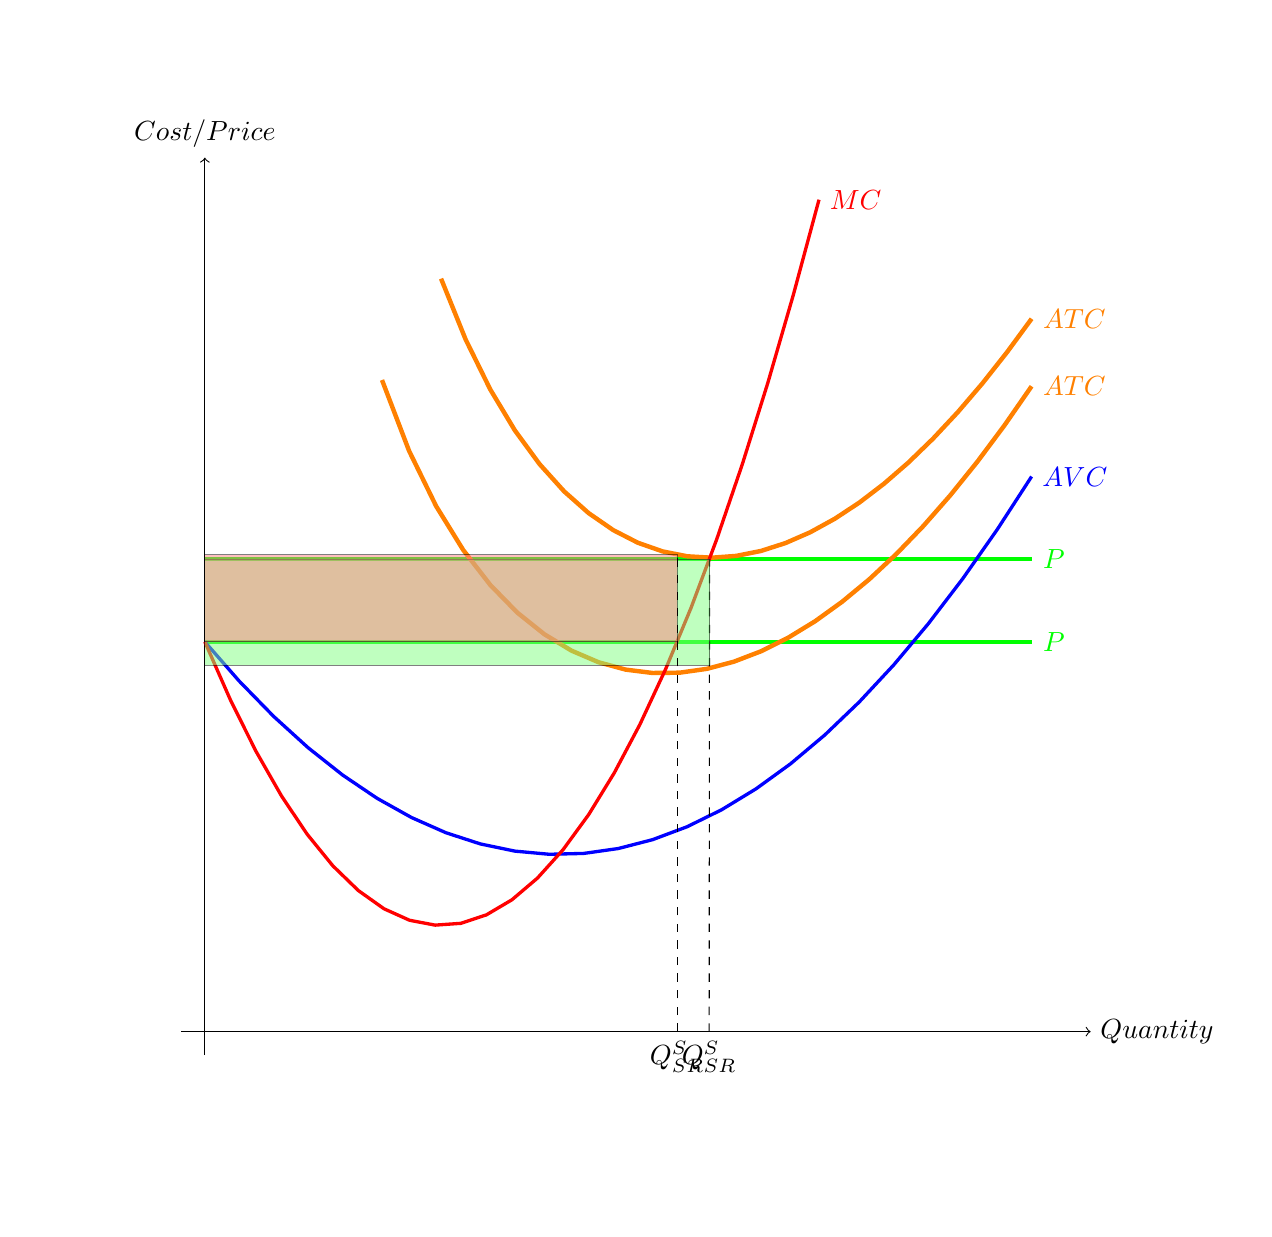
\begin{tikzpicture}[x=1.5cm, y=1.5cm]
  % Clip drawing region to y <= 12
  \clip (-1.5,-1.5) rectangle (8.8,8.5);

  % \draw[very thin,color=gray,style=dashed] (-0,-0) grid (7.1,6.5);

  \draw[->] (-0.2,0) -- (7.5,0) node[right] {$Quantity$};
  \draw[->] (0,-0.2) -- (0,7.4) node[above] {$Cost/Price$};

  % short run price
  \vary{
  \draw[ultra thick, color=green] (0,4)  -- (7,4) node[right] {$P$};
  }{
  \draw[ultra thick, color=green] (0,3.3)  -- (7,3.3) node[right] {$P$};
  }

  % cost curves
  \vary{
  \draw[ultra thick, color=orange, domain=1.5:7] plot (\x,{0.2*\x^2 - 1.2*\x + 3.3 + 5.35 / \x}) node[right] {$ATC$}; 
  }{
  \draw[ultra thick, color=orange, domain=2:7] plot (\x,{0.2*\x^2 - 1.2*\x + 3.3 + 9.35 / \x}) node[right] {$ATC$}; 
  }
  \draw[very thick, color=blue, domain=0:7] plot (\x,{0.2*\x^2 - 1.2*\x + 3.3}) node[right] {$AVC$}; 
  \draw[very thick, color=red, domain=0:5.2] plot (\x,{0.6*\x^2 - 2.4*\x + 3.3}) node[right] {$MC$}; 

  % solutions
  \PrintSolutionsTF{
    \vary{
      \draw[style=dashed] (4.27,0) node[below] {$Q^S_{SR}$} -- (4.273,4);
      \filldraw[fill=green!50, semitransparent] (0,3.1) rectangle (4.273,4);
    }{\draw[style=dashed] (4,0) node[below] {$Q^S_{SR}$} -- (4,4.0375);
      \filldraw[fill=red!50, semitransparent] (0,3.3) rectangle (4,4.0375);
    }
  }{}
\end{tikzpicture}


\PrintSolutionsTF{
  \fbox{\parbox{\linewidth}{
    \begin{itemize}
      \item The profit maximizing level of quantity supplied in the short run $Q_{SR}^S$ is where $P=MR$ intersects $MC$.
      \item \vary{In the short-run here, the firm's $MR>ATC$, so their profits are \textbf{positive}.

      On the graph this is the shaded rectangle which has a height of $P-ATC$ and a width of $Q_{SR}^S$.
      In the long-run other firms would \textbf{enter} until the price was driven \textbf{down} to the minimum of the $ATC$ 
      and all firms would be earning zero profit.
      }{In the short-run here, the firm's $ATC>MR$, so their profits are \textbf{negative}.

      On the graph this is the shaded rectangle which has a height of $ATC-P$ and a width of $Q_{SR}^S$.
      In the long-run other firms would \textbf{exit} until the price was driven \textbf{up} to the minimum of the $ATC$ 
      and all firms would be earning zero profit.}
    \end{itemize}
    }
  }
  }{\vspace{5cm}}

\end{question}